\section{Critical Core Radius}\label{crit_radius}

Neutronic viability is an important part of reactor design. The figure of merit
for neutronics is EOL \keff. The reactor must be able to sustain a fission
chain reaction from startup to shutdown on the final day of the 10 year mission.

The criticality requirement is the second of two major criteria for a valid reactor design and an
important constraint in the thermal hydraulic modeling process. As a result,
modeling criticality of various reactor configurations demands its own chapter
in this thesis. Criticality modeling started with depletion modeling, reported
in Section \ref{sec:sweeps}. The purpose and conclusion of the depletion
modeling was that thermal power and small geometric features were of low
importance when predicting EOL \keff. In addition, higher enrichment will always
be prefferred to lower enriched uranium.

The thermal-hydraulic modeling scheme
reported in Section \ref{sec:mass_model} requires a constraint for the core
radius. A relationship between core radius and fuel fraction for a target
value of \keff was developed using traditional reactor physics tools. In lieu of
full depletion modeling, BOL \keff was modeled and the \keff target adjusted to
ensure sufficient excess reactivity for 10 years of full-power operation.

There were three major components to developing the critical core radius
constraints, determining a value for BOL excess reactivity that would satisfy
EOL \keff > 1, generating the relationship between fuel fraction and the
required core radius to meet the target \keff value. For each fuel fraction, an
optimized reflector thickness was also calculated to minimize total core mass.
It is worth noting that critical core radius is a
bit of a misnomer, since the target of this analysis was a BOL excess
reactivity.

This process will be described in full for a single reactor core. The process
was performed for additional combinations of coolants and fuels and in theory,
could be applied to future reactor concepts. For simplicity of explanation, the
\uox-\codiox reactor will be used to demonstrate the neutronics optimization
workflow.

\subsection{Excess Reactivity}
As discussed in Section \ref{sec:sweeps}, EOL \keff is weakly dependent on
thermal power. This means that EOL \keff can be modeled as BOL \keff with enough
excess reactivity to account for depletion. With a target BOL reactivity,
depletion neutronics can be modeled with simple criticality calculations. This
is important because traditional depletion tools are too computationally
expensive to explore the desired reactor parameter space. Excess reactivity was
chosen based on the reactivity change in each of the 3901. Figure
\ref{fig:delta_k_eol} shows the reactivity swing $(\delta k$) for every core
with 100 kg < core mass < 500 kg. These bounds were chosen by initial analysis
showing the reactor design would fall in this domain.

\begin{figure}[h]
    \centering
    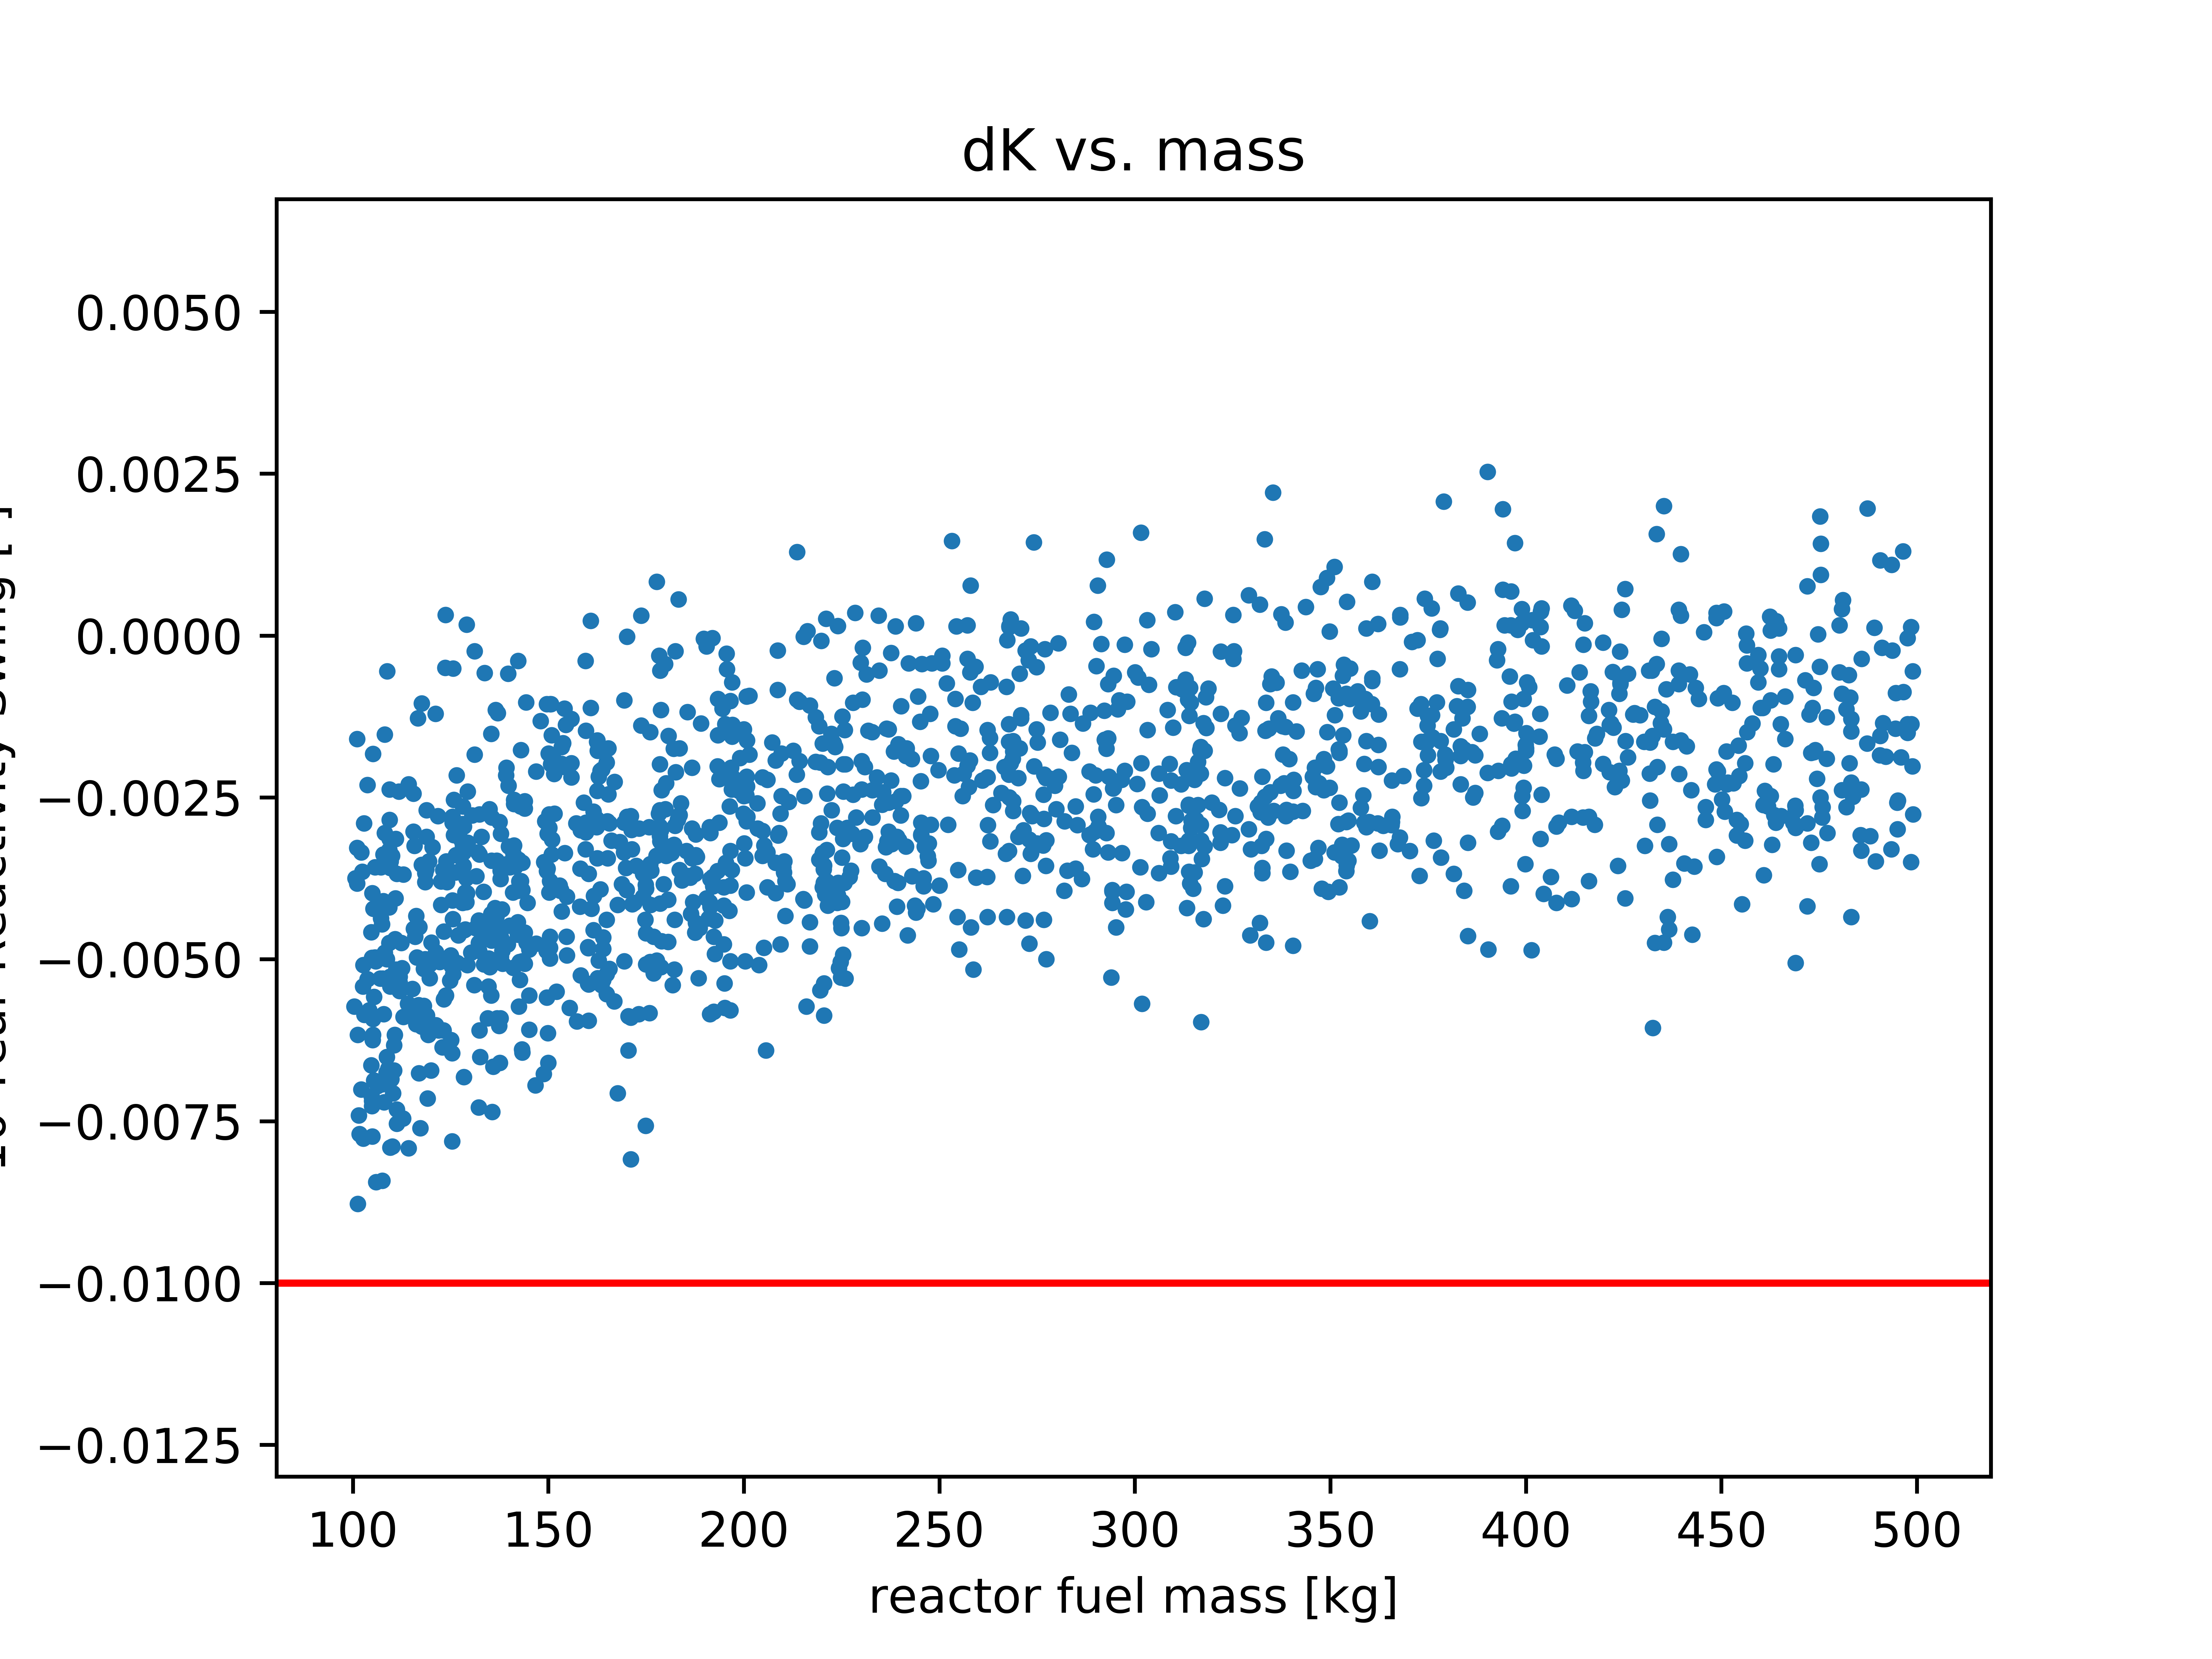
\includegraphics[width=4in]{../images/dK_vs_mass.png}
\caption{Reactivity swing over reactor lifetime}
\label{fig:delta_k_eol}
\end{figure}

A BOL \keff of 1.01 was deemed sufficient to sustain the fission chain reaction
through 10 years of full-power operation. This \keff target was used to define a
critical core radius, and to optimize the reflector thickness multipliers
(discussed in the following sections).

\subsection{Criticality Modeling}\label{sec:crit_model}
In order to constrain the reactor mass model, a critical radius relationship to
fuel fraction was developed. This section discusses the methods used to derive a
relationship between critical core radius and fuel fraction that was used by the
reactor mass model.

\subsubsection{Modeling Methods}
Section \ref{sec:sweeps} explored reactor parameter space to determine the
important predictors for EOL \keff. It was concluded that BOL \keff with
sufficient excess reactivity is an acceptable surrogate for EOL \keff. This was
an important conclusion because it significantly reduced the required
computation to model EOL \keff. Depletion calculations with traditional reactor
physics software are computationally expensive and slow. In contrast,
criticality calculations converge quickly and results can be returned much
faster. Three predictor variables were explored to model BOL \keff: core radius,
fuel fraction, and reflector mulitplier. The reflector multiplier being the
reflector radius defined as a multiplier of core radius. Equation
\ref{eq:ref_mult} shows the reflector radius as a function of core radius and
reflector multiplier.

\begin{equation}
    \label{eq:ref_mult}
    R_{refl} = mR_{core}
\end{equation}

Core radius, fuel fraction, and reflector multiplier all impact \keff.
Increasing the core radius adds more fuel mass and decreases neutron leakage 
from the core. Increasing fuel fraction also increases fuel mass, increasing
absorption cross sections in the fuel and decreasing leakage from the core.
Finally, adding reflector thickness prevents neutrons from leaking from the
core. All of these inputs are proportional to increasing BOL \keff. To model
their impact, a 3-dimensional grid of sampling data was generated. For each
point in 3d (radius, frac, multiplier) space, a criticality calculation was
performed using MCNP6.1

\subsubsection{Criticality Models}
The \keff response to the three modeled parameters was generated on a grid using
MCNP6.1 criticality models. The models were homogeneous geometries consisting of
a core region (fuel, cladding, and coolant), a reflector region (graphite), a
pressure vessel (SS-304), and finally the surronding Martian regolith. The top of the
reflector was buried 1 m below the surface of the Martian regolith. Figure
\ref{fig:homog_model} shows an example reactor geometry.

\begin{figure}[h]
    \centering
    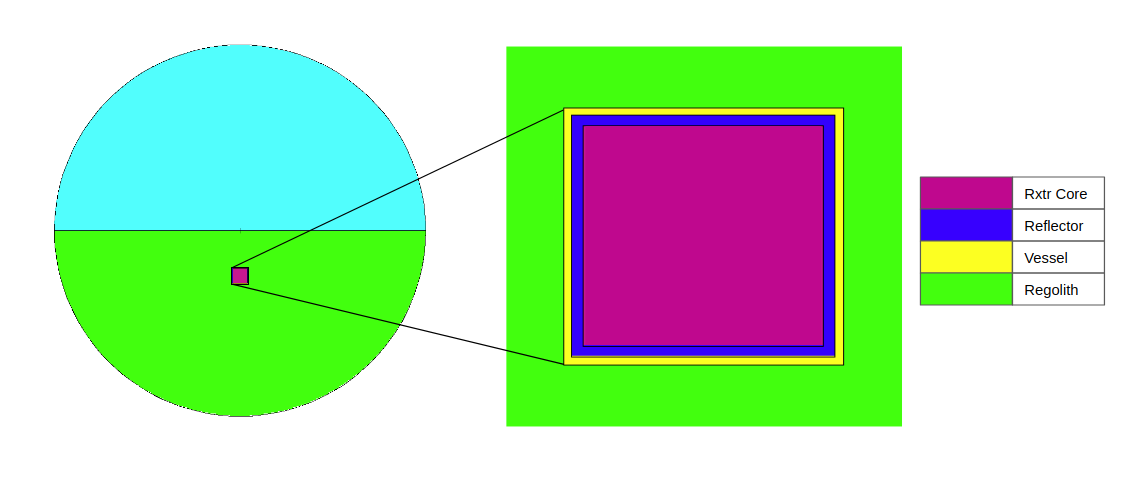
\includegraphics[width=4in]{../images/crit_model_geom.png}
\caption{Example reactor criticality model.}
\label{fig:homog_model}
\end{figure}

The reactor model and surronding Martian soil was modeled in a sphere. Vaccuum
boundary conditions were imposed on the edge of the sphere. Physically, neutrons
that reach the edge of the sphere are extremely unlikely to return to the core
and induce a fission, this is typical neutronics modeling practice.

Every \keff calculation was performed at room temperature. Neutron absorption
due to doppler broadening in 
\urantwo was assumed negligible due to high enrichment. A higher energy
spectrum due to no moderation also increass the resonance escape probability.
This assumption was checked in later neutronics verification calculations. 
In the end, BOL excess reactivity was chosen such that it overcame any 
temperature-induced reactivity losses. 

\subsubsection{Parameter Ranges}

Initial scoping calculations were performed to determine appropriate ranges for
each of the three parameters (radius, frac, and multiplier). 1000 kcode
calculations were run on a 10x10x10 grid, evenly sampling in each dimension.
Table \ref{tab:bol_criticality_1000} shows the sampled domain for the initial
scoping calculation.

\begin{table}[h]
  \centering
  \caption{Criticality Sampling Domain}
  \begin{tabular}{ll}
    \toprule
     Core Radius            		   & 10 - 50 [cm] \\
     Fuel Fraction 					   & 0.1 - 0.95 [-]\\
     Reflector Multiplier			   & 0.001- 1.5 [-]\\
  \end{tabular}
  \label{tab:bol_criticality_1000}
\end{table}

Each of these 1000 data points were used to generate a 3D \keff response to
core radius, fuel fraction, and reflector multiplier. This data set was used to
generate a set of mass-optimized reactors constrained to a target BOL \keff of
1.01. Section \ref{sec:crit_rad_search} discusses the algorithm used to generate
the minimized, constrained reactor masses.

\subsection{Critical Mass Optimization}\label{sec:crit_rad_search}
Section \ref{sec:crit_modeling} described the process for modeling the \keff
response to three input variables. It was necessary to determine a response
function to describe \keff for any combination of radius, fuel fraction, and
reflector multiplier so that \keff could be constrained to a BOL excess
reactivity target. The generalized function desired was:

\begin{equation}
    k_{eff} = f(r, f, m)
\label{eq:gen_keff}
\end{equation}

Where r is core radius, f is fuel fraction, and m is reflector multiplier. This
function would be used to constrain the models to the required \keff target. All
mass-minimized reactors were forced to satisfy this constraint.

\subsubsection{Modeling Criticality Results}
Linear interpolation was used to develop a function for \keff to be used to
constrain the core geometry. SciPy's 'RegularGridInterpolator' package was used
to generate a callable function in Python. This function used the grid data
generated in Section \ref{sec:crit_rad_search} to return \keff as a function of
r, f, and m. Trilinear interpolation was used to estimate the \keff response.
Trilinear interpolation perfomrs a linear combination of the 8 nearest points in
a cube surronding the desired point of interpolation. Linear interpolation is
only continuous to the zeroth derivative, but for large data sets, provides a
fast-executing function to model \keff.

Linear interpolation is a great tool for modeling data sets in between grid
values. It can be easily implemented using packages like SciPy. Scipy's grid
interpolator can be stored as a python object and rapidly executed like any
python function, making it useful as the target function for a mass
optimization. Despite numerous pratical advantages for using a trilinear
interpolator, there is systemic error introduced into the optimization by
representing nonlinear curves as piecewise-linear functions. The grid
interpolator was tested in order to understand the magnitude of this induced
error. A testing set of data was generated in the same domain space as the data
used to train the interpolator. This data was generated using Latin Hypercube
Sampling instead of being spaced evenly on the grid. LHS ensured that every
point would a check for the interpolator that did not contain data directly from
the grid. The testing set was 500 \keff results. For each \keff result in the
testing data, an interpolated result was generated using an interpolation
function (created from the training data). The absolute error was calculated
between each test \keff and its corresponding interpolated \keff. Figure
\ref{fig:interp_check} shows the distribution of error.

\begin{figure}[h]
    \centering
    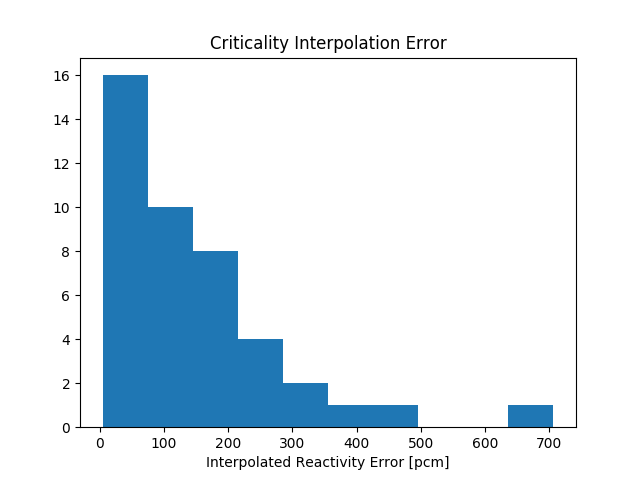
\includegraphics[width=4in]{../images/check_interp.png}
\caption{Histogram results of the reactivity discrepancy between interpolated
and real data.}
\label{fig:interp_check}
\end{figure}

\subsubsection{Critical Core Radius}
Core radius was used as a free variable to meet the \keff constraint target. For
a given fuel fraction and reflector multiplier, a core radius exists that meets
the target \keff. At the heart of this workflow is Equation \ref{eq:gen_keff}
and its representation as a trilinear interpolation function. This function was
used to interrogate the \keff response to varying core radii at fixed fuel
fractions and reflector masses. SciPy's 'minimize scalar' package was used to
perform this search. The goal of the search is to minimize the absolute error
between the interpolated \keff and the target \keff.

\begin{equation}
    min( (k(r, f, m) - k_0)^2 )
\end{equation}

For a fixed fuel fraction and reflector multiplier, 'minimize scalar' performs a
bounded optimization to return a valid core radius to meet the target \keff
constraint. This routine is executed in a Python function called 'crit radius'.
This function was used in multiple steps to optimize the reactor mass.

\subsubsection{Critical Mass Optimization}
With a routine in place to constrain core radius to a target \keff, an
optimization to minimize mass was performed. Recall from Section
\ref{sec:mass_model}, the goal of the neutronics modeling was to provide a
critical constraint for core radius as a function of fuel fraction. For each
fuel fraction, the thermal hydraulic mass model needs a core radius that
minimizes the core mass. The reflector multiplier (m) was used as the free
variable to optimize overall core mass. 

Reflectors impact neutronics by reflecting neutrons back into the core. This
reflection reduces leakage and improves the neutron economy, as a result,
reflected reactor cores require less fuel mass than bare cores. Increasing the
thickness of the reflector helps to a point, eventually adding more reflector
mass does not improve neutronic performance. Neutron leakage of course, is only
one part of the neutron life cycle, there are diminishing neutronic returns to
reflector thickness. In addition to improving the neutron economy, increasing
the reflector size increases the mass of the overall reactor. The tradeoff
between reflector mass and fuel mass was explored with the objective of
minimizing total reactor mass. 

Reflector thickness optimization was performed using the critical radius
workflow discussed previously. The goal of the optimization was to produce a
valid, critical core, with an optimized reflector thickness to minimize the
overall reactor mass. For every fuel fraction, a set of 20 multipliers was
checked from 0 to 0.16. For each multiplier, a critical radius search was
performed. The total mass (fuel, reflector, pressure vessel) for each critical
reactor was fitted against the reflector multipliers with a 2nd degree
polynomial. This polynomial was used as a target function for SciPy's
'minimize scalar' to minimize the core mass in reflector multiplier space.

The goal of the reflector optimization was to minimize the overall reactor mass
as a function of reflector multiplier for a fixed fuel fraction and a core
radius constrained to a \keff target. The optimization is performed over a range
of fuel fractions, for each fuel fraction, the optimized reflector is used to
generate a critical core radius that optimizes total reactor mass.


\subsubsection{Critical Mass Optimization Results}

The critical mass optimization in reflector multiplier space was performed for
each reactor configuration. The following is the results of the \uox fueled,
\codiox cooled reactor.

\begin{figure}[h]
    \centering
    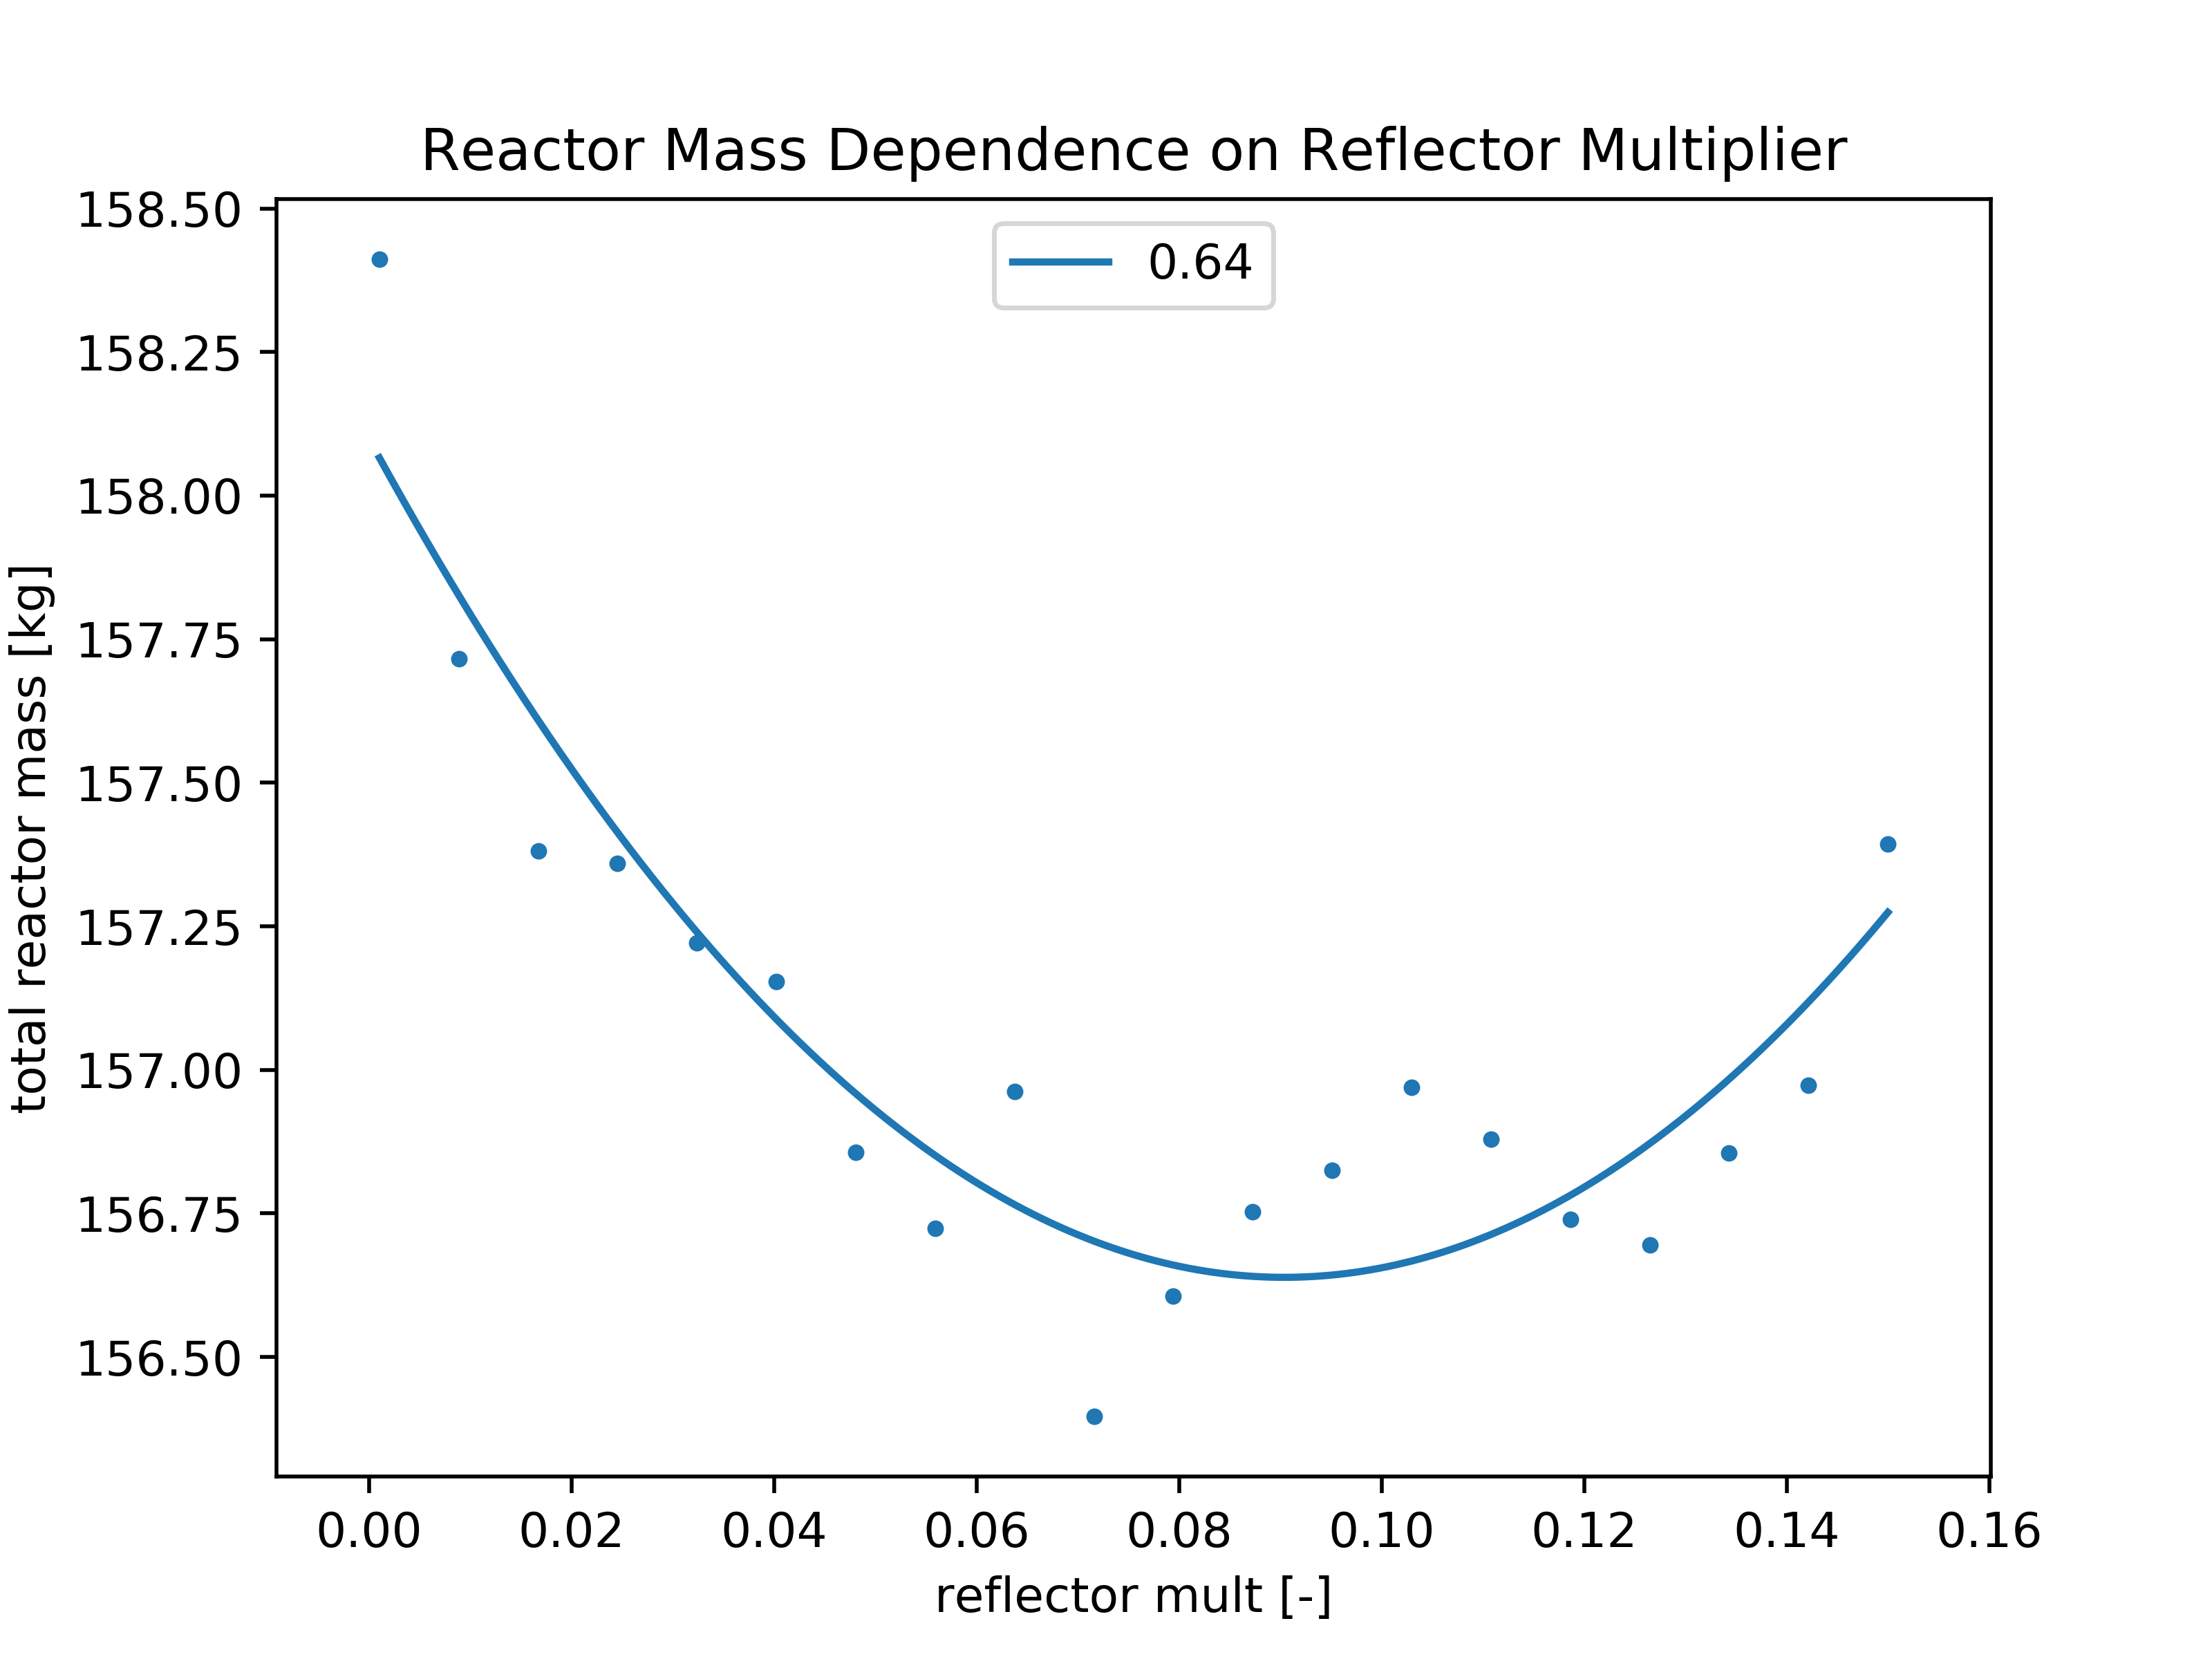
\includegraphics[width=4in]{../images/mass_mult_064.png}
\caption{Total reactor mass optimization for fuel fraction of 0.64}
\label{fig:mass_mult_one}
\end{figure}

Figure \ref{fig:mass_mult_one} shows the result of this optimization for one
fuel fraction, 0.64 for a UO2-CO2 reactor configuration. An important takeaway here, is the lack of curvature in
this plot. The reactor mass for this configuration is relatively insensitive to
reflector thickness. This is likely due to the HEU fuel providing a much
stronger absorption cross section, resulting in less leakage from the core. In
addition to strong fuel absorption, the reactor is buried in the Martian
regolith, some reflection can be expected from the soil around the reactor.
The standard deviation of the critical masses across reflector multiplier space
further indicates that reflector thickness is unimportant for the overall mass
optimization.

\begin{figure}[h]
    \centering
    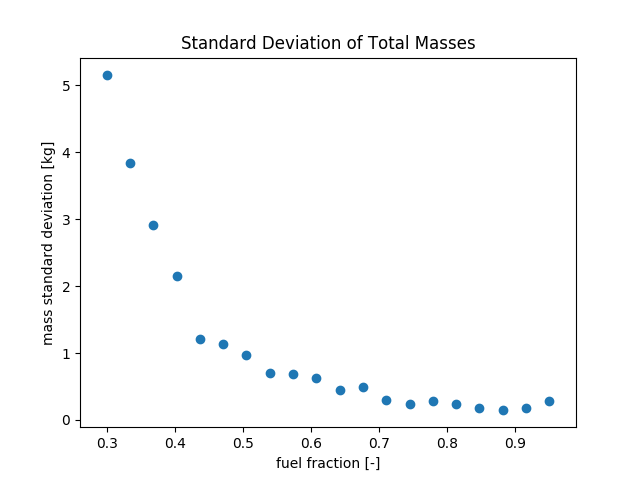
\includegraphics[width=4in]{../images/mass_std_uo2_co2.png}
\caption{Standard deviation of reactor mass in reflector multiplier space}
\label{fig:mass_std_co2_uo2}
\end{figure}

The standard deviation of the mass across the range of tested reflector
multipliers is very small relative to the size of the overall power cycle. As a
result, for the \uox-\codiox configuration, reflector multiplier was fixed to an
average value of 0.08. This average value was used to generate a critical radius
curve as a function of fuel fraction. This curve is used by the thermal
hydraulic reactor mass model to constrain the radius of the core for a given
fuel fraction. 

\begin{figure}[h]
    \centering
    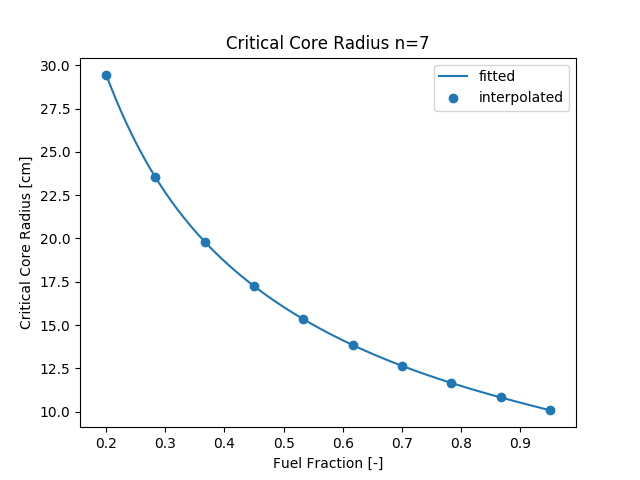
\includegraphics[width=4in]{../images/uo2_co2_core_r.png}
\caption{Critical radius dependence on fuel fration.}
\label{fig:core_r_co2_uo2}
\end{figure}


